\documentclass{article}[18pt]
\usepackage{../../../../../format}
\lhead{CT - Bioinformatics}


\begin{document}
\begin{center}
\underline{\huge Lecture 1}
\end{center}
\section{Big Data}
What is big data
\begin{itemize}
	\item Volume - Quantity of data
	\item Velocity - Speed at which data is collected
	\item Variety - Data in different formats
\end{itemize}
DNA sequence data can be considered "Big" in terms of volume. To cope with this we need to:
\begin{itemize}
	\item Build large efficient databases
	\item Develop fast and accurate algorithms
	\item Develop visualisation tools to help understand and interpret large data sets
\end{itemize}
\section{Tree Construction}
\begin{enumerate}
	\item Extract DNA sequence from each species
	\item Align the sequences
	\item Compute the inter-species distances
	\item Build the tree from the distance matrix
\end{enumerate}
\section{Sequence alignment}
\begin{center}
	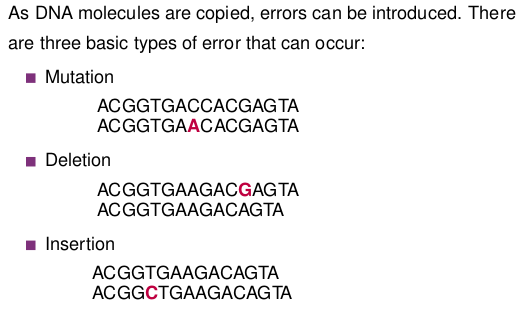
\includegraphics[scale=0.7]{sequence_alignment}
\end{center}
These errors rarely occur alone. It is likely we will see all of these errors when comparing two sequences.\\
\\
Let us compare the following sequences:
\begin{center}
	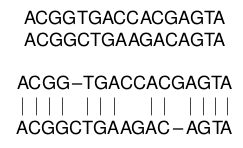
\includegraphics[scale=0.7]{alignment}
\end{center}
\begin{itemize}
	\item How do we go about trying to align two sequences
	\item We can insert gaps into the sequences to align them better, and then use a scoring algorithm
	\item You score:
	\begin{itemize}
		\item +1 for each position in which the sequences agree
		\item -1 for each position in which the sequences disagree
	\end{itemize}
\end{itemize}
Example. Align the two sequences
\end{document}